\documentclass{report}
\usepackage{graphicx}
\usepackage{listings}
%\usepackage{fullpage}

\begin{document}

% \documentclass[12pt]{article}

% \usepackage{ngerman}
% \selectlanguage{ngerman}
% \usepackage[latin1]{inputenc}

% \usepackage{graphicx}

% \begin{document}

\pagestyle{empty}

\begin{center}

\vspace*{-2.8cm}
\begin{minipage}[c]{.30\textwidth}
  \begin{flushleft}
    
\includegraphics[width=3cm,clip=]{LOGO/new-aerlogo.eps}%
  \end{flushleft}
\end{minipage}
\begin{minipage}[c]{.43\textwidth}
    { ~\\ Lehrstuhl f\"{u}r Aerodynamik \\ Prof.~Dr.-Ing. N.~A.~Adams}%
\end{minipage}
\begin{minipage}[c]{.25\textwidth}
  \begin{flushright}
    \vspace*{1em}
    
\includegraphics[width=3cm,clip=]{LOGO/TUMLogo_oZ_Vollfl_blau_RGB.eps}%
  \end{flushright}
\end{minipage}

\vspace*{3.3cm}
\begin{minipage}[c]{11cm}
{\LARGE\bf 
A Riemann solver }
\end{minipage}

\vspace*{0.8cm}
Mark F\"{o}rster\\

\vspace*{2.8cm}
{\bfseries Diplomarbeit}

\vspace*{1.2cm}
%\large
\normalsize
\vfill
\begin{tabular}{ll}
Betreuer: &  Dr.-Ing. Christian Stemmer \\
\ & \ \\
Ausgabe: & 1.\ Oktober 2008\\
Abgabe: & 31.\ M\"{a}rz 2009\\
\end{tabular}

\vspace*{1.6cm}
%\large
Lehrstuhl f\"{u}r Aerodynamik an der Technischen Universit\"{a}t M\"{u}nchen\\
2009
\end{center}

\pagebreak
\pagestyle{plain}

%\end{document}



\tableofcontents
\chapter{Introduction}
\label{sec:intro}
To test bibliography~\cite{Monaghan2005}

\chapter{Method}
\label{sec:method}


\lstinputlisting[language=c++,caption=An example of program listing,captionpos=b]{code/hello.cpp}


\chapter{Results}
\label{sec:results}

In the Figure~\ref{fig:1dshock} one can see \ldots

\begin{figure}[h]
  \centering
  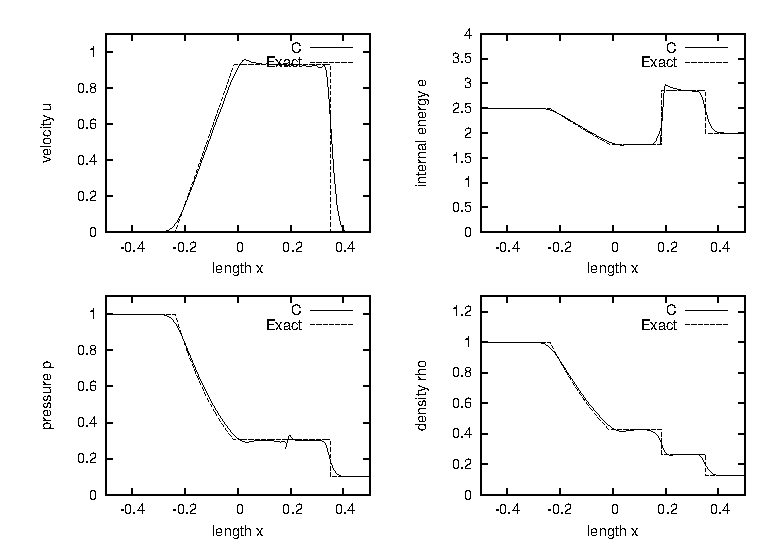
\includegraphics[width=0.95\textwidth]{img/1dshock.eps}
  \caption{An example of a figure}
  \label{fig:1dshock}
\end{figure}




\chapter{Conclusion}
\label{sec:conclusion}

\listoffigures

\bibliography{bibdata}
\bibliographystyle{plain}

\end{document}

